\documentclass[tikz,border=8pt]{standalone}
% Style commun des schémas : thème clair / sombre (couleurs des thèmes GitHub), fond transparent.
\usepackage[T1]{fontenc}
\usepackage{tgheros}
\renewcommand{\familydefault}{\sfdefault}
\usepackage{tikz}
\usetikzlibrary{positioning,arrows.meta,calc,fit,backgrounds}
\ifdefined\darktheme
  \definecolor{fg}{HTML}{E6EDF3}  \definecolor{muted}{HTML}{9198A1}
  \definecolor{line}{HTML}{8B949E} \definecolor{boxfill}{HTML}{151B23}
  \definecolor{boxline}{HTML}{3D444D}
  \definecolor{blue}{HTML}{4493F8} \definecolor{orange}{HTML}{DB6D28}
  \definecolor{green}{HTML}{3FB950} \definecolor{red}{HTML}{F85149}
  \definecolor{purple}{HTML}{AB7DF8}
\else
  \definecolor{fg}{HTML}{1F2328}  \definecolor{muted}{HTML}{59636E}
  \definecolor{line}{HTML}{59636E} \definecolor{boxfill}{HTML}{F6F8FA}
  \definecolor{boxline}{HTML}{D1D9E0}
  \definecolor{blue}{HTML}{0969DA} \definecolor{orange}{HTML}{BC4C00}
  \definecolor{green}{HTML}{1A7F37} \definecolor{red}{HTML}{CF222E}
  \definecolor{purple}{HTML}{8250DF}
\fi
\tikzset{
  every node/.style={text=fg, font=\small},
  block/.style={draw=boxline, fill=boxfill, rounded corners=3pt, line width=0.7pt,
                minimum height=11mm, minimum width=30mm, align=center, inner sep=5pt},
  sub/.style={font=\scriptsize, text=muted},
  wire/.style={line width=1pt, -{Stealth[length=2.6mm]}},
  biwire/.style={line width=1pt, {Stealth[length=2.6mm]}-{Stealth[length=2.6mm]}},
  lbl/.style={font=\scriptsize, text=muted, fill=none, inner sep=2pt},
}

\begin{document}
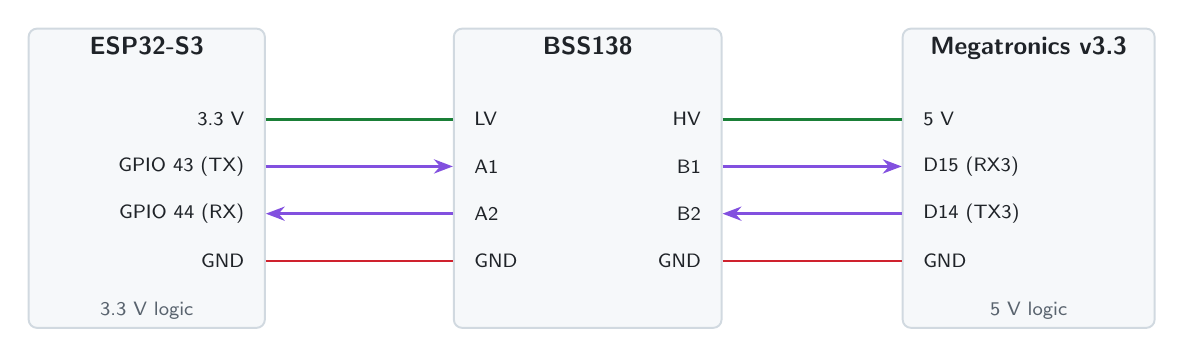
\begin{tikzpicture}
  \node[block, minimum width=30mm, minimum height=38mm] (esp) at (0,0) {};
  \node[font=\small\bfseries, anchor=north] at (esp.north) {ESP32-S3};
  \node[sub, anchor=south] at (esp.south) {3.3 V logic};
  \node[block, minimum width=34mm, minimum height=38mm] (bss) at (5.6,0) {};
  \node[font=\small\bfseries, anchor=north] at (bss.north) {BSS138};
  \node[block, minimum width=32mm, minimum height=38mm] (mega) at (11.2,0) {};
  \node[font=\small\bfseries, anchor=north] at (mega.north) {Megatronics v3.3};
  \node[sub, anchor=south] at (mega.south) {5 V logic};
  \foreach \y/\l/\lv/\hv/\r/\c/\st in {0.75/3.3 V/LV/HV/5 V/green/-, 0.15/GPIO 43 (TX)/A1/B1/D15 (RX3)/purple/{-{Stealth[length=2.4mm]}}, -0.45/GPIO 44 (RX)/A2/B2/D14 (TX3)/purple/{{Stealth[length=2.4mm]}-}, -1.05/GND/GND/GND/GND/red/-}{
    \node[font=\scriptsize, anchor=east] at ([xshift=-1.5mm]esp.east |- 0,\y) {\l};
    \node[font=\scriptsize, anchor=west] at ([xshift=1.5mm]bss.west |- 0,\y) {\lv};
    \node[font=\scriptsize, anchor=east] at ([xshift=-1.5mm]bss.east |- 0,\y) {\hv};
    \node[font=\scriptsize, anchor=west] at ([xshift=1.5mm]mega.west |- 0,\y) {\r};
    \draw[line width=1pt, \c, \st] (esp.east |- 0,\y) -- (bss.west |- 0,\y);
    \draw[line width=1pt, \c, \st] (bss.east |- 0,\y) -- (mega.west |- 0,\y);
  }
\end{tikzpicture}
\end{document}
